\subsection{Software in the Loop (SITL)}\label{subsection:E}
In executing the SITL simulation, a detailed virtual environment was established in the Gazebo simulator to closely mimic real-world conditions. This environment included models like buildings and trees, sourced directly from the Gazebo library. Additionally, to recreate an accurate geographical setting, a plane was generated using satellite imagery from the Google Maps API \cite{2e1}. This incorporation of real-world geographic data and physical objects greatly improved the authenticity of the simulated environment.

Additionally, human models were crafted using MakeHuman, a sophisticated tool designed to create realistic human avatars, and were subsequently rendered with Blender software. The files exported from MakeHuman included a mesh model, texture images, and a UV map — which is a flat representation of the 3D model used to map textures. All these components were imported into Blender to produce the final 3D rendered model. A demonstration of the human model creation process using MakeHuman and Blender is presented in Figure ~\ref{fig2e1}. This method provided lifelike representations of humans, which is essential for the drone's person re-identification capabilities.


\begin{figure}[H]
    \centerline{\includegraphics[width=0.5\textwidth]{Figures/Methods/makehuman+blender.png}}
    \caption{Human Model Creation Process: (left) MakeHuman / (right) Blender}
    \label{fig2e1}
\end{figure}

The centerpiece of the simulation was the Iris quadcopter model, equipped with a camera and a LiDAR sensor. The integration of these sensors into the Iris quadcopter model was crucial for the autonomous drone to navigate and recognize humans within the simulated environment accurately. A sample of the fully integrated world is illustrated in Figure \ref{fig2e2}.   

\begin{figure}[H]
    \centerline{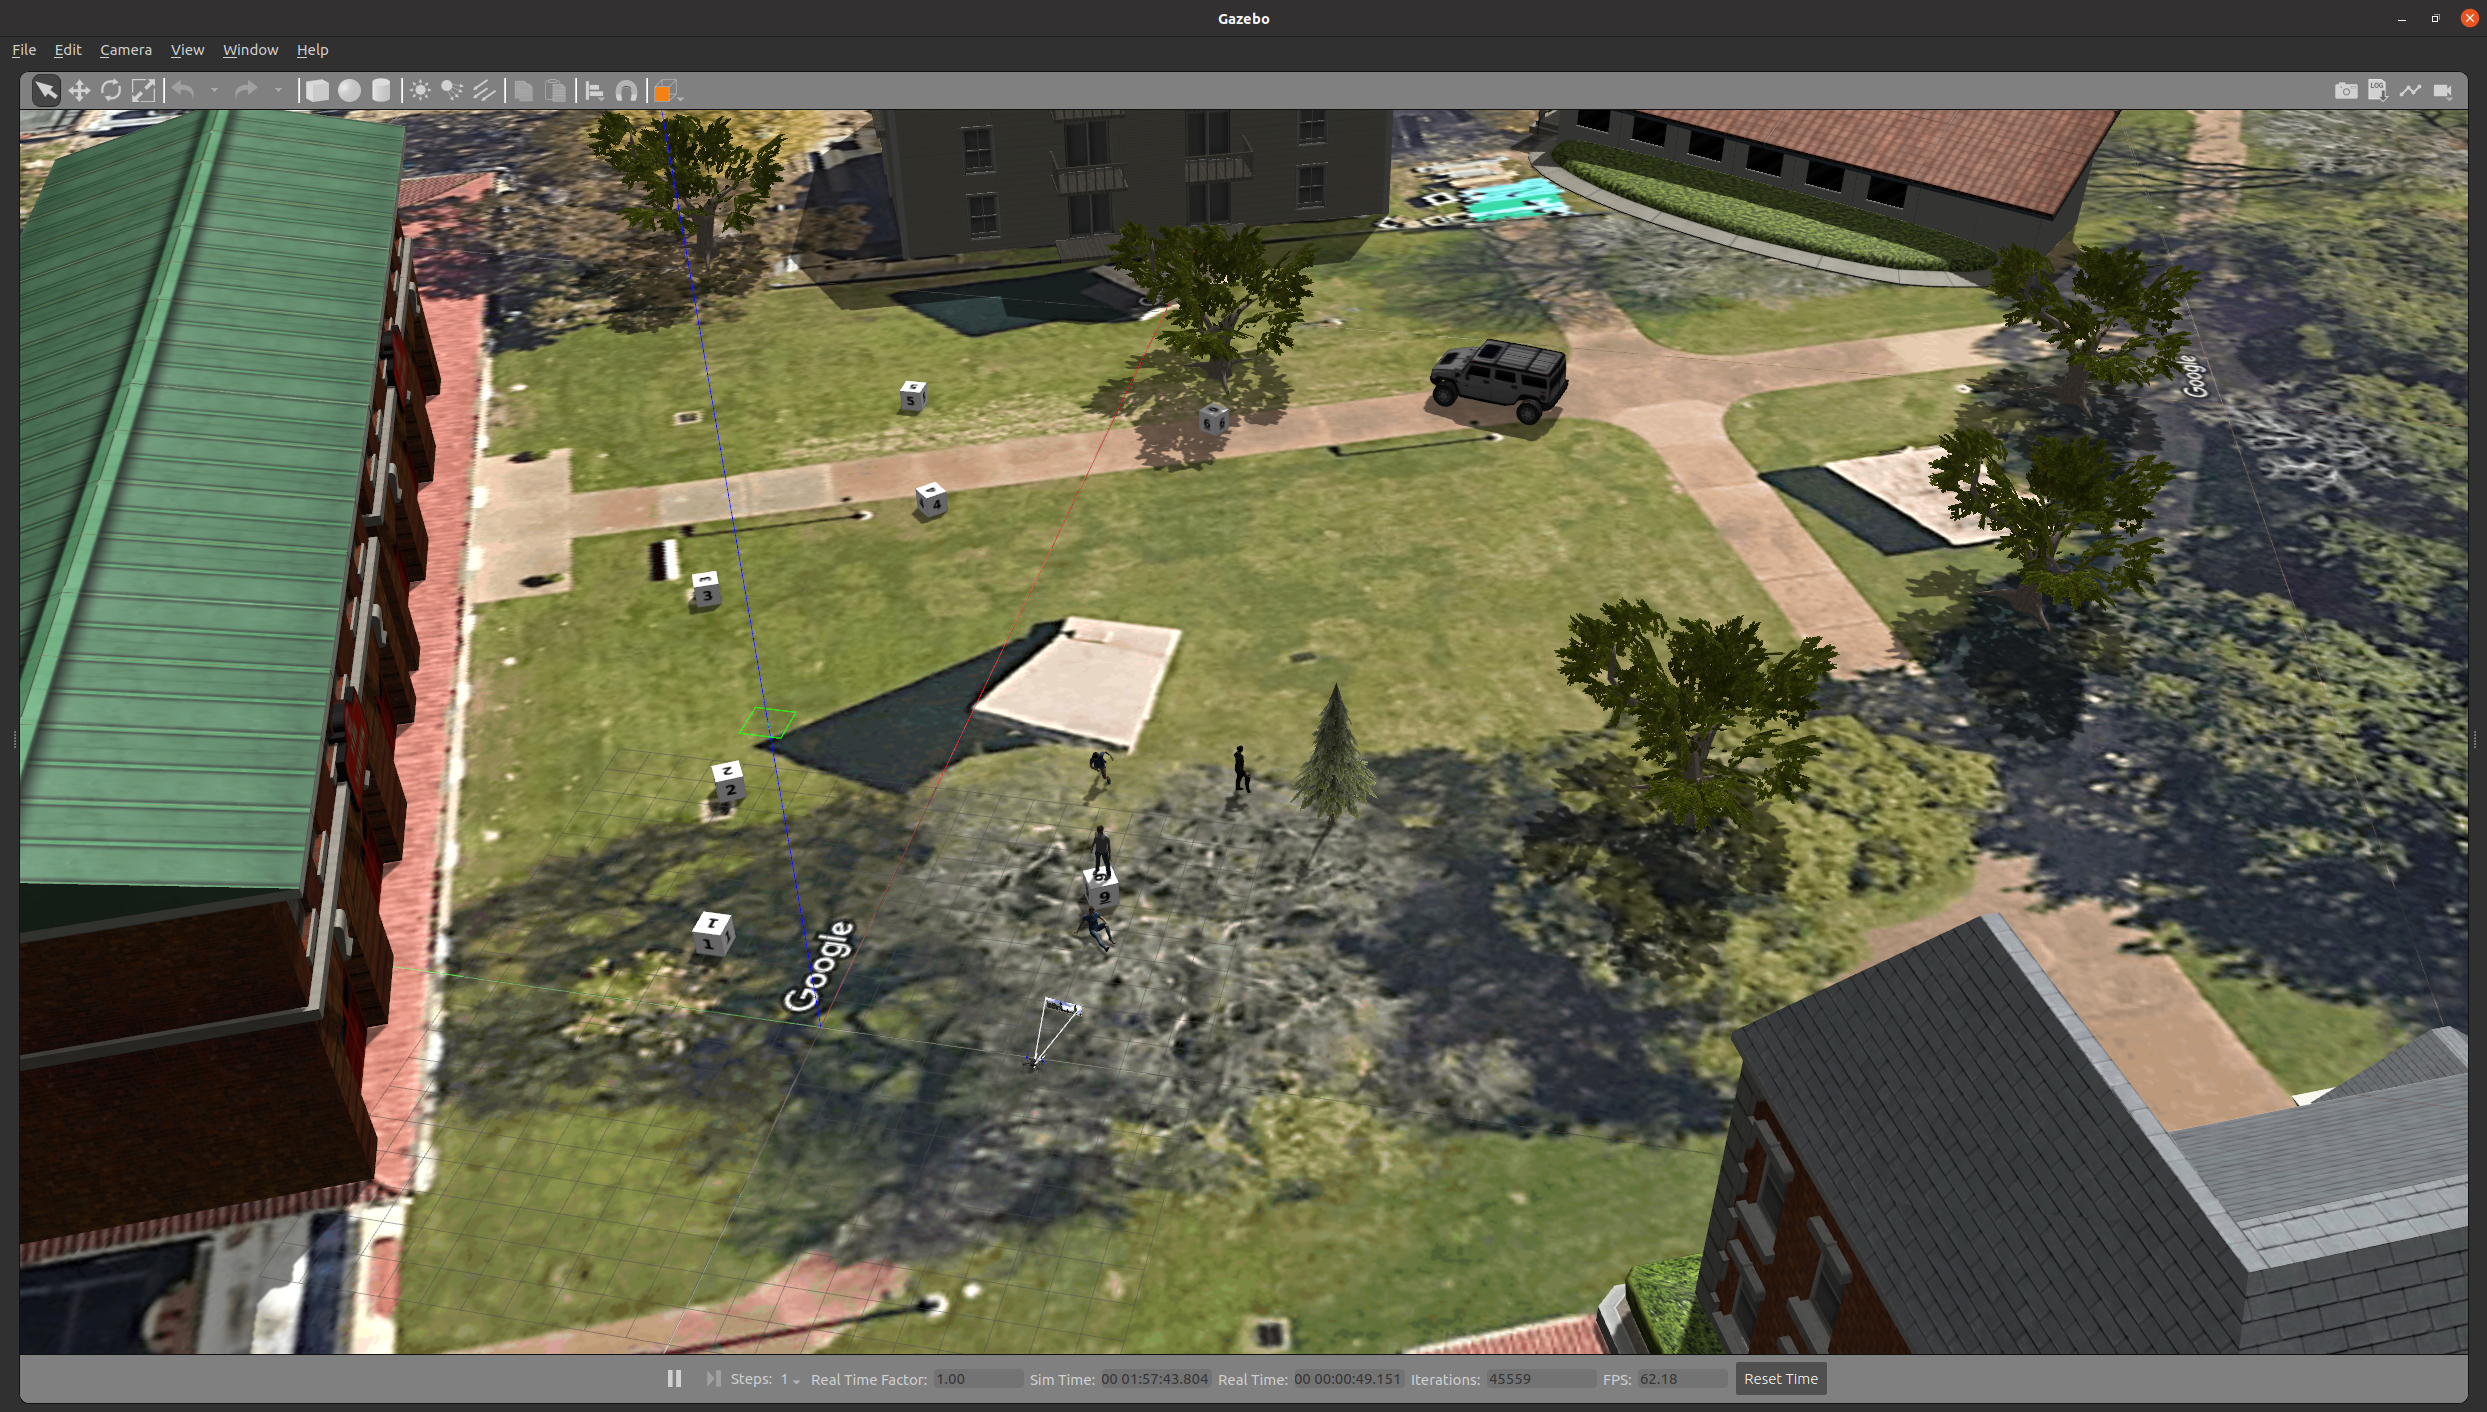
\includegraphics[width=0.5\textwidth]{Figures/Methods/env.png}}
    \caption{Gazebo World Environment}
    \label{fig2e2}
\end{figure}

Ardupilot's SITL is essential in the setup of the simulation for the project. It simulates the flight control hardware for the quadcopter in Gazebo and establishes a bridge to the ROS environment. The block diagram shown in Figure \ref{fig2e3} illustrates the communication pathway between the drone's Flight Control Unit (FCU) within Ardupilot's SITL and the Gazebo simulation environment, facilitated by the Gazebo Driver and MAVProxy. Gazebo handles the simulation of the drone's physical responses and sensor inputs, which are then interfaced with the ROS environment through ROS topics. ROS, in turn, sends control signals to the FCU using the MAVLink protocol via UDP ports. This process coordinates the drone's simulated activities and completes the loop of the integrated simulation system.

\begin{figure}[H]
    \centerline{\includegraphics[width=0.5\textwidth]{Figures/Methods/sitl_block_diagram.png}}
    \caption{SITL Block Diagram}
    \label{fig2e3}
\end{figure}

In developing the autonomous drone's control and object detection functionalities, specific libraries were selected for optimal performance and system compatibility. The "gnc\textunderscore functions" library from Intelligent Quads was chosen for drone control\cite{2e2}. It provides a comprehensive set of guidance, navigation, and control (GNC) functions made for autonomous drones, which enables precise maneuvering and stable flight. For object detection, the OpenCV deep neural network (DNN) module was used. The shift from Python to C++ for enhanced performance led to the selection of OpenCV's DNN module, which is well-suited for C++ environments. This module, particularly effective in real-time object detection, was utilized to load the ONNX YOLO model.


The integration of various simulation tools and models played a key role in developing a robust and realistic testing environment for the autonomous drone. This foundation is crucial for the drone's successful application in real-world scenarios.